\documentclass[a4paper,11pt,twocolumn]{article}
%\documentclass[twocolumn,aps,pre,groupedaddress]{revtex4-1}

\usepackage{amsmath}
\usepackage{graphicx}
\usepackage{amsmath}
\usepackage{graphicx}
\usepackage{subfig}
\usepackage{epstopdf}
\usepackage{amssymb}

\begin{document}
\title{Time Series Leanings}
\author{James M. McCracken}
%\email{jmccrac1@masonlive.gmu.edu}
%\affiliation{School of Physics, Astronomy, and Computational Sciences \\ George Mason University \\ 4400 University Drive MS 3F3, Fairfax,VA. 22030-4444}
\author{Robert S. Weigel}
%\email{rweigel@gmu.edu}
%\affiliation{School of Physics, Astronomy, and Computational Sciences \\ George Mason University \\ 4400 University Drive MS 3F3, Fairfax,VA. 22030-4444}
\date{\today}

%\begin{abstract}
%\end{abstract}

%\pacs{}
\maketitle

\section{Introduction}

\section{Causal Penchant}
Define the {\em causal penchant} as
\begin{equation}
\label{eq:pen}
\rho_{EC} := P\left(E|C\right) - P\left(E|\bar{C}\right)\;\;.
\end{equation}
The motivation for this expression is in te interpretation of $\rho_{EC}$ as a causal indicator; i.e.\ if $C$ causes (or {\em drives}) $E$, then $\rho_{EC} > 0$, and if $\rho_{EC} \le 0$, then the direction of causal influence in the system is undetermined.  If the effect $E$ is assumed to be recorded in one time series and the cause $C$ is assumed to be recorded in a different time series, then the direction of causal influence in the system can be determined by comparing various penchants calculated using both time series.  The details of these comparison is discuss in the following sections, but some potential philosophical issues with this definition will be addressed first.

$\ldots$ {\em {\bf Add discussion of Pearl argument that $P(E|\bar{C})$ is ''unobservable''.}}

Pearl's concerns can be addressed by rewriting Eqn.\ \ref{eq:pen} using the law of total probability, i.e
\begin{equation}
\label{eq:totp}
P(E) = P(E|C)P(C) + P(E|\bar{C})P(\bar{C})\;\;,
\end{equation}
or Bayes theorem, i.e.\ 
\begin{equation}
\label{eq:bayes}
P(E|\bar{C}) = P(\bar{C}|E)\frac{P(E)}{P(\bar{C})}\;\;.
\end{equation}
The definition of probability complements implies $P(\bar{C}) = 1-P(C)$ and $P(\bar{C}|E) = 1-P(C|E)$.  Applying Eqn.\ \ref{eq:bayes} leads to
\begin{equation}
P(\bar{C}|E) = 1-P(E|C)\frac{P(C)}{P(E)}
\end{equation}
Thus,
\begin{equation}
P(E|\bar{C}) = \left(1-P(E|C)\frac{P(C)}{P(E)}\right)\frac{P(E)}{1-P(C)}\;\;.
\end{equation}
This expression implies
\begin{equation}
\ref{eq:pencal}
\rho_{EC} = P(E|C)\left(1+\frac{P(C)}{1-P(C)}\right)-\frac{P(E)}{1-P(C)}
\end{equation}
This same expression can be derived without Eqn.\ \ref{eq:bayes} by using Eqn.\ \ref{eq:totp} to make the appropriate substitution for $P(E|\bar{C})$ into Eqn.\ \ref{eq:pen}.

The use of either Eqn.\ \ref{eq:totp} or Eqn.\ \ref{eq:bayes} may eliminate the concern that $P(E|\bar{C})$ is fundamental unobservable.  It may also, however, introduce new philosophical concerns in the definition of the penchant.  For example, $\ldots$ {\em {\bf expand this discussion}}

It follows from Eqn.\ \ref{eq:pen} that
\begin{equation}
\rho_{EC}\in\left[1,-1\right]\;\;,
\end{equation}
but, more importantly for the calculations in the following sections, the penchant is not defined if $P(C)$ or $P(\bar{C})$ are zero (because the conditionals in Eqn.\ \ref{eq:pen} would be undefined).  Thus, the penchant is not defined if $P(C)=0$ or if $P(C)=1$.  The former condition is interpreted intuitively as an inability to determine causal influence between two time series using points that do not appear in one of the series, and the latter condition is interpreted intuitively as an inability to determine causal influence between two time series if one of the data series is constant.  The use of Bayes theorem in the derivation of Eqn.\ \ref{eq:pencal} implies that same conditions apply to $P(E)$.  It will be seen below that there is no {\em a priori} assignments of ''cause'' or ''effect'' to a given time series when using penchants for causal inference.  So, operationally, these conditions of $P(C)$ and $P(E)$ only mean that the penchant is undefined between pairs of time series where one series is constant. 

The philosophical concerns are perhaps not as important as an answer to the straightforward question of whether or not the penchant is a useful tool for time series causality.  The rest of this article will focus on answering that question.

\section{Mean Observed Leaning}
Consider
\begin{eqnarray*}
x &=& \left\{0,0,2,0,0,2,0,0,2,0\right\}\\
y &=& \left\{0,0,0,2,0,0,2,0,0,2\right\}
\end{eqnarray*}
and a penchant defined as
$$
\rho_{y_{t}x_{t-1}} = P\left( y_t = 2 | x_{t-1} = 2\right) - P\left( y_t = 2 | x_{t-1} \neq 2\right)
$$
Estimating the probabilities with frequency counts is straightforward for the first term, i.e.\
$$
P\left( y_t = 2 | x_{t-1} = 2\right) = \frac{n_{EC}}{n_C} = \frac{3}{3} = 1\;\;,
$$
where $n_{EC}$ is the number of times $y_t=2$ and $x_{t-1}=2$ appears in the pair of time series (where, in this case, $y_t$ is assumed to be the effect $E$ caused by the cause $C$, $x_{t-1}=2$) and $n_{C}$ is the number of times the assumed cause, $x_{t-1}=2$, has appeared.  The conditional probability $P(A|B)$ is not defined if $P(B) = 0$, thus $n_C >0$ by definition, and $n_{EC}<=n_C$ because even though the assumed effect, $y_t=2$, might occur without the assumed cause, $x_{t-1}=2$ in the data, the count $n_{EC}$ is defined to be when they occur together.  It follows that this definition of $P\left( y_t = 2 | x_{t-1} = 2\right)$ can be interpreted as a probability.  

The second term in the penchant is trickier.  Consider the following frequency count,
$$
P\left( y_t = 2 | x_{t-1} \neq 2\right) = \frac{n_{EnC}}{n_{nC}} = \frac{0}{6} = 0\;\;,
$$
where $n_{EnC}$ is the number of times the assumed effect, $y_t=2$ appears given that the assumed cause $x_{t-1}=2$ has {\em not} occurred, i.e.\ $x_{t-1}\neq 2$, and $n_{nC}$ is the number of times the assumed cause $x_{t-1}=2$ has {\em not} occurred, i.e.\ the number of times $x_{t-1}\neq 2$.  There are seven zeros in $\{x_t$\}, so it may be assumed that $n_{nC}=7$ rather than $n_{nC}=6$ as used above.  But, the condition is on $x_{t-1}$, not $x_t$.  Thus, the time series actually being compared are
\begin{eqnarray*}
\tilde{x} &=& \left\{0,0,2,0,0,2,0,0,2\right\}\\
\tilde{y} &=& \left\{0,0,2,0,0,2,0,0,2\right\}
\end{eqnarray*}
which are both shorter than there counterparts above by a single value.  It follows that $\tilde{x}_t = x_{t-1}$ and $\tilde{y}_t=y_t$.  This subsetting of the time series will be discussed again later.

Again, this definition can be interpreted as a probability (for very similar reason to those mentioned above).  However, this term can be rewritten using Bayes' theorem or the law of total probability as
$$
P\left( y_t = 2 | x_{t-1} \neq 2\right) = \frac{P\left( y_t = 2 \right)}{P\left( x_{t-1} \neq 2 \right)} - P\left( y_t = 2 | x_{t-1} = 2\right)\frac{P\left( x_{t-1} = 2 \right)}{P\left( x_{t-1} \neq 2 \right)}\;\;.
$$
Substituting the frequency counts leads to
$$
P\left( y_t = 2 | x_{t-1} \neq 2\right) = \frac{n_E}{n_{nC}} - \frac{n_{EC}}{n_C}\frac{n_C}{n_{nC}} = \frac{3}{6} - \frac{3}{3}\frac{3}{6} = 0\;\;,
$$
where the only frequency seen here but not used above is $n_E$ the number of times the assumed effect $y_t=2$ has appeared.  Also consider the completeness relation $P\left( x_{t-1} \neq 2 \right) = 1 - P\left( x_{t-1} = 2 \right)$.  This substitution leads to
$$
P\left( y_t = 2 | x_{t-1} \neq 2\right) = \frac{P\left( y_t = 2 \right)}{1-P\left( x_{t-1} = 2 \right)} - P\left( y_t = 2 | x_{t-1} = 2\right)\frac{P\left( x_{t-1} = 2 \right)}{1-P\left( x_{t-1} = 2 \right)}
$$
and
$$
P\left( y_t = 2 | x_{t-1} \neq 2\right) = \frac{n_E}{1-n_{C}} - \frac{n_{EC}}{n_C}\frac{n_C}{1-n_{C}} = \frac{3}{3} - \frac{3}{3}\frac{3}{3} = 0\;\;.
$$
The last expression has removed any reference to $P\left( x_{t-1} \neq 2 \right)$ and $n_{nC}$, which might be considered unobservable.  This particular penchant is the same for both calculation methods.

Consider both these calculation methods for all the possible penchants in this pair of time series, i.e.\
\begin{center}
\begin{tabular}{c|c|c|c|c|c}
$\rho_{y_{t}x_{t-1}}$ & $P(E|C)$ & $P(E|\bar{C})$ method 1 & $P(E|\bar{C})$ method 2 & result 1 & result 2\\
\hline
 $y_{t}=2,x_{t-1}=2$& 1 & 0 & 0 & 1 & 1\\
 $y_{t}=2,x_{t-1}=0$& 0 & 1 & 1 & -1 & -1\\
 $y_{t}=0,x_{t-1}=2$& 0 & 1 & 1 & -1 & -1\\
 $y_{t}=0,x_{t-1}=0$& 1 & 0 & 0 & 1 & 1
\end{tabular}
\end{center}
For this example, both methods are equal for all the penchants.  The main concern here is that the second conditional probability term in the definition of the penchant has been replaced with probabilities of the assumed causes and effects.  This substitution addresses the argument that this second conditional probability term is not observable (e.g.\ Pearl's argument that there's no way to know what an effect given ``no cause'' actually is supposed to mean).  However, it introduces concerns about the underlying assumption that the assumed cause must precede the assumed effect.  This concern is partially addressed by subsetting $\{x\}$ and $\{y\}$ into $\{\tilde{x}\}$ and $\{\tilde{y}\}$ because for any given $t$, $\tilde{x}_t$ precedes $\tilde{y}_t$.  But, once is this assumptions still true when frequency counts are used to estimate the necessary probabilities; e.g.\ when $P(x_{t-1}=0)$ and $P(y_t=0)$ are estimated above, is it sufficient to use   
$$
P(x_{t-1}=0) = \frac{n_{x0}}{L}
$$ 
and 
$$
P(y_t=0) = \frac{n_{y0}}{L}\;\;,
$$
where $n_{x0}$ is the number of times $\tilde{x}_t = 0$, $n_{y0}$ is the number of times $\tilde{y}_t = 0$, and $L$ is the library length of both $\{\tilde{x}\}$ and $\{\tilde{y}\}$?  The working assumption is yes, but the issue will be addressed primarily by testing the algorithm.

The algorithm used to calculate the penchants calculates only $\rho_{y_{t}=2,x_{t-1}=2}$ and $\rho_{y_{t}=0,x_{t-1}=0}$ but not $\rho_{y_{t}=2,x_{t-1}=0}$ and $\rho_{y_{t}=0,x_{t-1}=2}$ because the former are the only $(y_{t},x_{t-1})$ pairs that actually appear in the data.  The observed mean penchant is then 
$$
\bar{\rho}_{y_{t},x_{t-1}} = \frac{1}{2}\left( \rho_{y_{t}=2,x_{t-1}=2} + \rho_{y_{t}=0,x_{t-1}=0} \right) = 1\;\;,
$$
which implies the probability that $x_{t-1}$ drives $y_{t}$ is higher than the probability that it does not.  The observed mean leaning is then
$$
\bar{l}_{xy} = \bar{\rho}_{y_{t},x_{t-1}} - \bar{\rho}_{x_{t},y_{t-1}}\;\;,
$$
and the casual inference would be $\bar{l}>0\Rightarrow \mathbf{x}\rightarrow\mathbf{y}$, $\bar{l}<0\Rightarrow \mathbf{y}\rightarrow\mathbf{x}$, and $\bar{l}=0\Rightarrow ??$; i.e.\ a positive observed mean leaning implies $\mathbf{x}$ drives $\mathbf{y}$ more than $\mathbf{y}$ drives $\mathbf{x}$ with an analogous conclusion for a negative observed mean leaning.   

\subsection{Algorithm}

\section{Simple Example Systems}

\subsection{Impulse with Noisy Response Linear Example}
Consider the linear example dynamical system of
\begin{eqnarray}
\label{eq:linearex1}
X_t &=& \{0,2,0,0,2,0,0,2,0,0\}\\
Y_t &=& X_{t-1}+B\eta_t,
\end{eqnarray}
with $B\in\mathbb{R}\ge 0$ and $\eta_t\sim\mathcal{N}\left(0,1\right)$.  Specifically, consider $B\in[0,2]$ in increments of 0.02.  The response system $Y$ is just a lagged version of the driving signal with varying levels of standard Gaussian noise applied at each time step.  
\begin{figure}[ht]
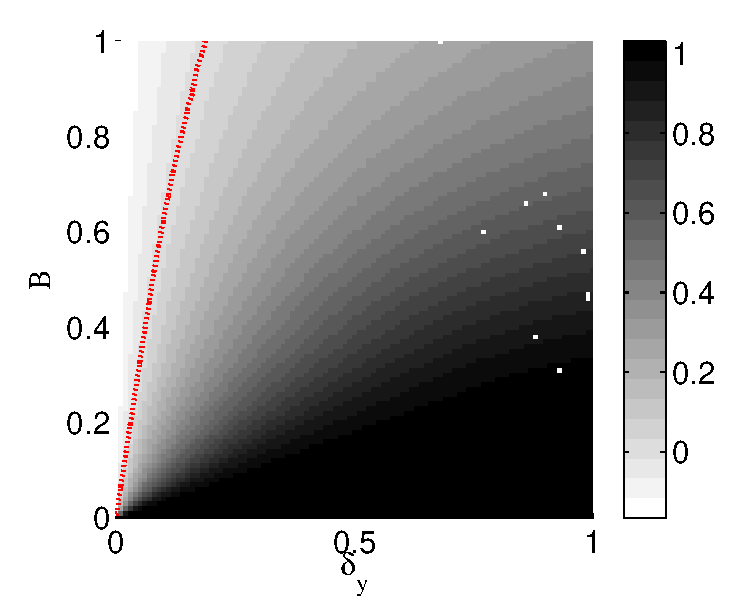
\includegraphics[scale=0.45]{SimpleIRexample_plot.eps}
\caption{Leaning as a function of both the noise and the y-tolerance.}
\end{figure}

\subsection{Cyclic Linear Example}
Consider the linear example dynamical system of
\begin{eqnarray}
\label{eq:linearex}
X_t &=& \sin(t)\\
Y_t &=& X_{t-1}+B\eta_t,
\end{eqnarray}
with $B\in\mathbb{R}\ge 0$ and $\eta_t\sim\mathcal{N}\left(0,1\right)$.  Specifically, consider $B\in[0,2]$ in increments of 0.02.  The response system $Y$ is just a lagged version of the driving signal with varying levels of standard Gaussian noise applied at each time step.  

\subsection{Non-Linear Example}
Consider the non-linear dynamical system of
\begin{eqnarray}
\label{eqn:nonlinearEX}
X_t &=& \sin(t)\\
Y_t &=& AX_{t-1}\left(1-BX_{t-1}\right)+C\eta_t,
\end{eqnarray}
with $A,B,C\in\mathbb{R}\ge 0$ and $\eta_t\sim\mathcal{N}\left(0,1\right)$.  Specifically, consider $A,B,C\in[0,5]$ in increments of 0.5.  

\subsection{RL Circuit Example}
\label{sec:rlcirc}
Both of the previous examples included a noise term, $\eta_t$.  Consider a series circuit containing a resistor, inductor, and time varying voltage source related by
\begin{equation}
\label{eqn:it}
\frac{dI}{dt} = \frac{V(t)}{L} - \frac{R}{L} I,
\end{equation}
where $I$ is the current at time $t$, $V(t)= \sin\left(\Omega t\right)$ is the voltage at time $t$, $R$ is the resistance, and $L$ is the inductance.  Eqn. \ref{eqn:it} was solved using the {\em ode45} integration function in MATLAB.  The time series $V(t)$ is created by defining values at fixed points and using linear interpolation to find the time steps required by the ODE solver.  

Consider the situation where $L=10$ Henries and $R=5$ Ohms are constant.  Physical intuition is that $V$ drives $I$, and so we expect to find that $V$ CCM causes $I$ (i.e., $C_{VI}>C_{IV}$ or $\Delta = C_{VI}-C_{IV} > 0$). 


\section{Empirical Data}

\section{Conclusion}

%\bibliographystyle{plain}
%\bibliography{main}

\end{document}